%% SECTION 5.3 %%
\section{Covering Numbers}

As pointed out in the previous section, we need a suitable generalization of VC theory to find a bound on the Rademacher complexity $\mathfrak{R}_n(l \circ \mathcal{F})$ for arbitrary (i.e., possibly infinite) function classes $\mathcal{F}$. We have seen that the cardinality of the set $T_l(z) = \{(l(f(x_1), y_1), \dots, l(f(x_n), y_n))^{\top} \with f \in \mathcal{F}\}$ plays a significant role in bounding the Rademacher complexity of $l \circ \mathcal{F}$. When $\mathcal{F}$ is infinite, the set $T_l(z)$ will  most likely be infinite as well. Thus, we need to find a way that lets us treat points in this set that are close to each other as if they were identical. The concept of \emph{$\varepsilon$-coverings} will help us do just that.

\begin{definition}
Let $(X, d)$ be a pseudometric space, let $K$ be a subset of $X$, and let $\varepsilon > 0$. An \emph{external $\varepsilon$-covering} of $K$ is a set $V \subset X$ such that
\[
    K \subset \bigcup_{x \in V} B_{d, \varepsilon}(x),
\]
where $B_{d, \varepsilon}(x) = \set{y \in X \with d(x, y) \leq \varepsilon}$ is the closed ball of radius $\varepsilon$ centered at $x \in X$. $V$ is called an \emph{internal $\varepsilon$-covering} of $K$, if $V \subset K$.

The \emph{external $\varepsilon$-covering number} $\mathcal{N}^{\text{ext}}(K, d, \varepsilon)$ of $K$ is the minimum number of elements needed to form an external $\varepsilon$-covering of $K$, i.e.,
\[
    \mathcal{N}^{\text{ext}}(K, d, \varepsilon) = \inf\set{\abs{V} \with V \text{ is an external } \varepsilon \text{-covering of } K}.
\]
An external $\varepsilon$-covering $V$ of $K$ is called \emph{minimal}, if $\abs{V} = \mathcal{N}^{\text{ext}}(K, d, \varepsilon)$. Finally, \emph{internal $\varepsilon$-covering numbers} $\mathcal{N}^{\text{int}}(K, d, \varepsilon)$ and \emph{minimal} internal $\varepsilon$-coverings are defined analogously.
\end{definition}

\begin{figure}
    \centering
    \begin{tikzpicture}
        \node[above right, inner sep=0] (image) at (0,0) {
            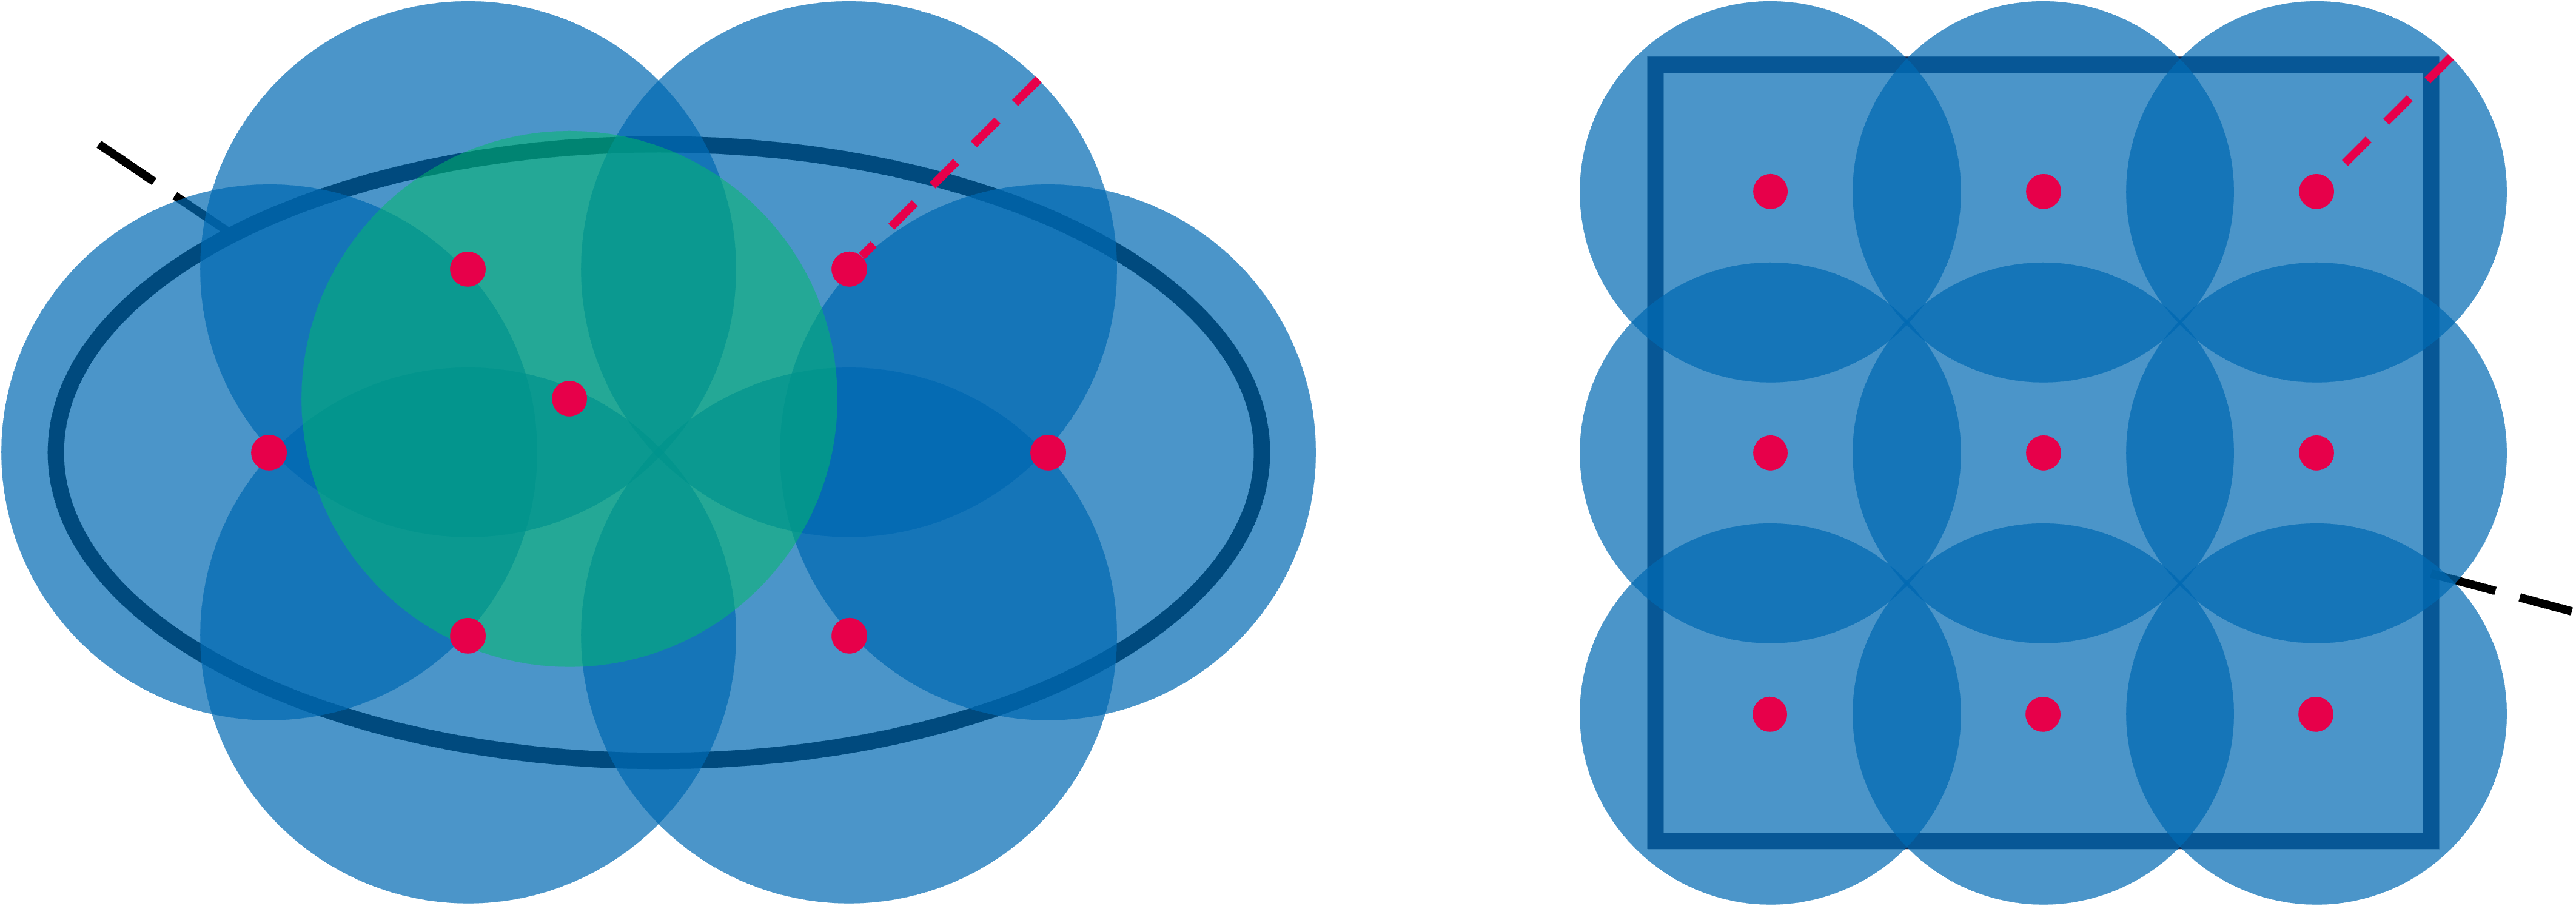
\includegraphics[width=13cm]{other/epsilon-covering}
        };

        % Create scope with normalized axes
        \begin{scope}[
            x={(image.south east)},
            y={(image.north west)}]
         
            % Grid to properly align annotations
            % \draw[help lines, step=0.1] (image.south west) grid ($(image.north east) + (0.001,0)$);

            % Annotate image
            \node[] at (0.02,0.86) {$\mathcal{F}_1$};
            \node[] at (0.36,0.90) {$\varepsilon_1$};
            \node[] at (0.09,0.46) {$g_1$};
            \node[] at (0.16,0.26) {$g_2$};
            \node[] at (0.31,0.26) {$g_3$};
            \node[] at (0.38,0.46) {$g_4$};
            \node[] at (0.31,0.66) {$g_5$};
            \node[] at (0.16,0.66) {$g_6$};
            \node[] at (0.20,0.52) {$g_7$};

            \node[] at (1.02,0.30) {$\mathcal{F}_2$};
            \node[] at (0.89,0.88) {$\varepsilon_2$};
            \node[] at (0.67,0.74) {$g_1$};
            \node[] at (0.77,0.74) {$g_2$};
            \node[] at (0.88,0.74) {$g_3$};
            \node[] at (0.67,0.46) {$g_4$};
            \node[] at (0.77,0.46) {$g_5$};
            \node[] at (0.88,0.46) {$g_6$};
            \node[] at (0.67,0.16) {$g_7$};
            \node[] at (0.77,0.16) {$g_8$};
            \node[] at (0.88,0.16) {$g_9$};
            
        \end{scope}
    \end{tikzpicture}
    \caption{%
         Coverings of two classes $\mathcal{F}_1$ and $\mathcal{F}_2$. \textbf{Left}, a class $\mathcal{F}_1$ covered by an $\varepsilon_1$-covering ${\color{red} V} = \set{{\color{red} g_1}, \dots, {\color{red} g_7}}$. Note, however, that $\mathcal{N}(\mathcal{F}, d, \varepsilon_1) < 7$ since the $\varepsilon_1$-ball centered at $g_7$ and depicted in green is redundant (i.e., the remaining 6 $\varepsilon_1$-balls still cover all of $\mathcal{F}_1$). \textbf{Right}, a class $\mathcal{F}_2$ covered by a \emph{minimal} $\varepsilon_2$-covering ${\color{red} V} = \set{{\color{red} g_1}, \dots, {\color{red} g_9}}$.
    }
    \label{fig: epsilon-covering}
\end{figure}

If $V$ is an $\varepsilon$-covering (external or internal) of a set $K$, then every $y \in K$ is within distance of at most $\varepsilon$ to some $x \in V$, i.e., for every $y \in K$ there exists $x \in V$ such that $d(x, y) \leq \varepsilon$. For a class of functions $\mathcal{F}$, we will assume $\varepsilon$-coverings to be \emph{internal} coverings, unless explicitly stated otherwise. To ease notation, we simply write $\mathcal{N}(\mathcal{F}, d, \varepsilon)$ for the internal $\varepsilon$-covering numbers.

Next, we introduce the \emph{conditional Rademacher average} of a class\footnote{In what follows, we use a general class of functions $\mathcal{F}$ and a set of points $\set{z_1, \dots, z_n}$. In the setting of empirical risk minimization, we would substitute $\mathcal{F}$ for $l \circ \mathcal{F}$ and the set under consideration would be the observations $\set{(x_1, y_1), \dots, (x_n, y_n)}$.} of functions $\mathcal{F}$ given a set of points $\set{z_1, \dots, z_n}$.

\begin{definition}
The \emph{conditional Rademacher average} of a class $\mathcal{F}$ of functions $f \colon \mathcal{Z} \to \R$ given a tuple $z = (z_1, \dots, z_n) \in \mathcal{Z}^n$ is defined as
\[
    \hat{\mathfrak{R}}_n^z(\mathcal{F}) = \Exp\left[\sup_{f \in \mathcal{F}} \abs{\frac{1}{n} \sum_{i=1}^n \sigma_i f(z_i)}\right],
\]
where $\sigma_1, \dots, \sigma_n$ are i.i.d.\ $\Rad(\nicefrac{1}{2})$ random variables.
\end{definition}

Notice that, if $\mathcal{F}$ is a class of functions $f \colon \mathcal{Z} \to \R$, and we define the Rademacher complexity of $\mathcal{F}$ as\footnote{This is simply the generalization of Definition \ref{def: rademacher complexity for general loss} to an arbitrary class of functions $\mathcal{F}$.}
\[
    \mathfrak{R}_n(\mathcal{F}) = \sup_{z \in \mathcal{Z}^n} \Exp\left[\sup_{f \in \mathcal{F}} \abs{\frac{1}{n} \sum_{i=1}^n \sigma_i f(z_i)}\right],
\]
then clearly
\begin{equation}
\label{eq: rademacher complexity and conditional rademacher average}
    \highlightMath{
        \mathfrak{R}_n(\mathcal{F}) = \sup_{z \in \mathcal{Z}^n} \hat{\mathfrak{R}}_n^z(\mathcal{F}).
    }
\end{equation}

There is one more term we have to introduce before we state the first result of this section.

\begin{definition}
Given a tuple $z = (z_1, \dots, z_n) \in \mathcal{Z}^n$ and a class $\mathcal{F}$ of functions $f \colon \mathcal{Z} \to \R$, the \emph{empirical $L^1$-distance} between $f, g \in \mathcal{F}$ is given by
\[
    d_1^z(f, g) = \frac{1}{n} \sum_{i=1}^n \abs{f(z_i) - g(z_i)}.
\]
\end{definition}

With these definitions in place, we will prove an upper bound of the conditional Rademacher average of a class $\mathcal{F}$ that (besides the number of observations $n$) depends only on the $\varepsilon$-covering numbers of $\mathcal{F}$ with respect to the empirical $L^1$-distance $d_1^z$. In order for these (covering numbers) to be well-defined, we would have to show that the empirical $L^1$-distance defines a pseudometric on a given class $\mathcal{F}$ (since this is assumed to be the case in the definition of covering numbers presented earlier). This is indeed true, and it follows directly from the properties of the absolute value.

\begin{theorem}
\label{thm: bound on conditional rademacher average}
Let $\mathcal{F}$ be a class of functions $f \colon \mathcal{Z} \to [-1, 1]$. Then,
\[
    \hat{\mathfrak{R}}_n^z(\mathcal{F}) \leq \inf_{\varepsilon > 0} \left( \varepsilon + \sqrt{\frac{2 \log(2 \mathcal{N}(\mathcal{F}, d_1^z, \varepsilon))}{n}} \right), \quad z \in \mathcal{Z}^n.
\]
\end{theorem}

\begin{proof}
We can assume $\mathcal{N}(\mathcal{F}, d_1^z, \varepsilon) < \infty$, since the inequality is trivially true otherwise. Given $\varepsilon > 0$, we let $V_{\varepsilon}$ be a minimal $\varepsilon$-covering of $\mathcal{F}$, i.e., $\abs{V_{\varepsilon}} = \mathcal{N}(\mathcal{F}, d_1^z, \varepsilon) < \infty$. For every function $f \in \mathcal{F}$, there exists $f^{\circ} \in V_{\varepsilon}$ such that $d_1^z(f, f^{\circ}) \leq \varepsilon$. By the triangle inequality, we have
\[
    \hat{\mathfrak{R}}_n^z(\mathcal{F}) = \Exp\left[\sup_{f \in \mathcal{F}} \frac{1}{n} \abs{\sum_{i=1}^n \sigma_i f(z_i)}\right] \leq \Exp\left[\sup_{f \in \mathcal{F}} \frac{1}{n} \abs{\sum_{i=1}^n \sigma_i (f(z_i) - f^{\circ}(z_i))}\right] + \Exp\left[\sup_{f \in \mathcal{F}} \frac{1}{n} \abs{\sum_{i=1}^n \sigma_i f^{\circ}(z_i)}\right].
\]
The triangle inequality also implies
\[
    \frac{1}{n} \abs{\sum_{i=1}^n \sigma_i (f(z_i) - f^{\circ}(z_i))} \leq \frac{1}{n} \sum_{i=1}^n \abs{f(z_i) - f^{\circ}(z_i)} = d_1^z(f, f^{\circ}) \leq \varepsilon,
\]
since $\abs{\sigma_i} = 1$ almost surely. Hence,
\[
    \hat{\mathfrak{R}}_n^z(\mathcal{F}) \leq \varepsilon + \Exp\left[\sup_{f \in \mathcal{F}} \frac{1}{n} \abs{\sum_{i=1}^n \sigma_i f^{\circ}(z_i)}\right].
\]
As $f^{\circ} \in V_{\varepsilon}$, we obtain
\[
    \Exp\left[\sup_{f \in \mathcal{F}} \frac{1}{n} \abs{\sum_{i=1}^n \sigma_i f^{\circ}(z_i)}\right] = \Exp\left[\max_{g \in V_{\varepsilon}} \frac{1}{n} \abs{\sum_{i=1}^n \sigma_i g(z_i)}\right] = \mathfrak{R}_n(B),
\]
where $\mathfrak{R}_n(B)$ denotes the Rademacher complexity of the \emph{finite} set $B = \set{(g(z_1), \dots, g(z_n))^{\top} \with g \in V_{\varepsilon}} \subset \R^n$. Since every $g \in V_{\varepsilon} \subset \mathcal{F}$ takes values in $[-1, 1]$, we have $\max_{b \in B} \norm{b}_2 \leq \sqrt{n}$, and Lemma \ref{lem: bound on rademacher complexity of finite set} hence tells us that
\[
    \mathfrak{R}_n(B) \leq \sqrt{\frac{2 \log(2 \abs{B})}{n}} \leq \sqrt{\frac{2 \operatorname{log}(2 \abs{V_{\varepsilon}})}{n}} = \sqrt{\frac{2 \operatorname{log}(2 \mathcal{N}(\mathcal{F}, d_1^z, \varepsilon))}{n}},
\]
since $\abs{B} \leq \abs{V_{\varepsilon}} = \mathcal{N}(\mathcal{F}, d_1^z, \varepsilon)$. Altogether,
\[
    \hat{\mathfrak{R}}_n^z(\mathcal{F}) \leq \varepsilon + \Exp\left[\sup_{f \in \mathcal{F}} \frac{1}{n} \abs{\sum_{i=1}^n \sigma_i f^{\circ}(z_i)}\right] \leq \varepsilon + \sqrt{\frac{2 \operatorname{log}(2 \mathcal{N}(\mathcal{F}, d_1^z, \varepsilon))}{n}}.
\]
Since this is true for every $\varepsilon > 0$, we can take the infimum over $\varepsilon$ to arrive at the desired result.
\end{proof}

Observe that there is a trade-off in the upper bound of the previous result, since the $\varepsilon$-covering numbers $\mathcal{N}(\mathcal{F}, d_1^z, \varepsilon)$ of $\mathcal{F}$ increase as $\varepsilon$ decreases, and vice versa. 

We want to apply Theorem \ref{thm: bound on conditional rademacher average} to bound the estimation error of the empirical risk minimizer $\hat{f}$ of the class $\mathcal{F}$ of linear functions introduced in Example \ref{ex: linear functions f_a}. From Section \ref{subsec: empirical risk minimization for general loss function} and Section \ref{subsec: rademacher complexity for general loss function}, we know that the inequality
\begin{align*}
    L(\hat{f}) - L(\bar{f}) &\leq 2 \sup_{f \in \mathcal{F}} \abs*{\hat{L}_n(f) - L(f)} \\
    &< 2 \Exp[\sup_{f \in \mathcal{F}} \abs*{\hat L_n(f) - L(f)}] + \sqrt{\frac{2 \log(\delta^{-1})}{n}} \leq 4 \mathfrak{R}_n(l \circ \mathcal{F}) + \sqrt{\frac{2 \log(\delta^{-1})}{n}}
\end{align*}
holds with probability at least $1 - \delta$ for any $\mathcal{F}$. We also know that we can write
\[
    \mathfrak{R}_n(l \circ \mathcal{F}) = \sup_{z \in \mathcal{Z}^n} \hat{\mathfrak{R}}_n^z(l \circ \mathcal{F})
\]
by \eqref{eq: rademacher complexity and conditional rademacher average}, and Theorem \ref{thm: bound on conditional rademacher average} provides a way to bound the conditional Rademacher average $\hat{\mathfrak{R}}_n^z(l \circ \mathcal{F})$. Finally, we have to compute the covering numbers of the class $l \circ \mathcal{F}$ with respect to the empirical $L^1$-distance $d_1^z$. The following Lemma will be helpful in doing so:

\begin{lemma}
\label{lem: distance between linear functions f_a}
Let $\mathcal{F}$ be defined as in \eqref{eq: family of linear functions f_a}, and assume that the loss function $l \colon \R \times \R \to [0, 1]$ is Lipschitz in its first argument, i.e.,
\[
    \abs{l(u, y) - l(v, y)} \leq K \abs{u - v}, \quad u, v, y \in \R,
\]
for some Lipschitz constant $K > 0$. Then, for any two linear functions $f_a, f_b \in \mathcal{F}$, we have
\[
    d_1^z(l \circ f_a, l \circ f_b) \leq K \norm{a - b}_{\infty}, \quad z \in \mathcal{Z}^n.
\]
\end{lemma}

\begin{proof}
Because the loss function is $K$-Lipschitz in its first argument, we have
\[
    d_1^z(l \circ f_a, l \circ f_b) = \frac{1}{n} \sum_{i=1}^n \abs{l(f_a(x_i), y_i) - l(f_b(x_i), y_i)} \leq \frac{1}{n} \sum_{i=1}^n K \abs{f_a(x_i) - f_b(x_i)} = \frac{K}{n} \sum_{i=1}^n \abs{\langle a - b, x_i \rangle}.
\]
Applying H{\"o}lder's inequality, we obtain
\[
    \abs{\langle a - b, x_i \rangle} \leq \sum_{j=1}^d \abs*{(a - b)^{(j)} x_i^{(j)}} \leq \norm{a - b}_{\infty} \norm{x_i}_1 \leq \norm{a - b}_{\infty}, \quad i = 1, \dots, n.
\]
Hence, we conclude
\[
    d_1^z(l \circ f_a, l \circ f_b) \leq \frac{K}{n} \sum_{i=1}^n \abs{\langle a - b, x_i \rangle} \leq \frac{K}{n} \sum_{i=1}^n \norm{a - b}_{\infty} = K \norm{a - b}_{\infty}. \qedhere
\]
\end{proof}

An immediate consequence of the previous result is the following:

\begin{corollary}
\label{cor: bound on covering numbers of linear functions}
Assuming that the loss function $l \colon \R \times \R \to [0, 1]$ is $K$-Lipschitz in its first argument, the covering numbers of the class $l \circ \mathcal{F}$, where $\mathcal{F}$ is defined as in \eqref{eq: family of linear functions f_a}, satisfy
\[
    \mathcal{N}(l \circ \mathcal{F}, d_1^z, \varepsilon) \leq \mathcal{N}(B_{\infty}^d(1), d_{\infty}, \nicefrac{\varepsilon}{K}).
\]
\end{corollary}

\begin{proof}
The inequality holds if $\mathcal{N}(B_{\infty}^d(1), d_{\infty}, \nicefrac{\varepsilon}{K}) = \infty$. Hence, we assume $\mathcal{N}(B_{\infty}^d(1), d_{\infty}, \nicefrac{\varepsilon}{K}) < \infty$, and we let $V_{\varepsilon / K}$ be a minimal $\nicefrac{\varepsilon}{K}$-covering of $(B_{\infty}^d(1), d_{\infty})$. Then,
\[
    W_{\varepsilon} = \set{l \circ f_{a_0} \with a_0 \in V_{\varepsilon / K}}
\]
defines an $\varepsilon$-covering of $(l \circ \mathcal{F}, d_1^z)$. To see this, let $f_a \in \mathcal{F}$ be arbitrary, with $a \in B_{\infty}^d(1)$. Since $V_{\varepsilon / K}$ is an $\nicefrac{\varepsilon}{K}$-covering of $(B_{\infty}^d(1), d_{\infty})$, there exists $a_0 \in V_{\varepsilon / K}$ such that $d_{\infty}(a, a_0) \leq \varepsilon / K$. For $l \circ f_{a_0} \in W_{\varepsilon}$, this implies
\[
    d_1^z(l \circ f_a, l \circ f_{a_0}) \leq K \norm{a - a_0}_{\infty} = K d_{\infty}(a, a_0) \leq \varepsilon
\]
by Lemma \ref{lem: distance between linear functions f_a}. Therefore, $W_{\varepsilon}$ is an $\varepsilon$-covering of $(l \circ \mathcal{F}, d_1^z)$ with cardinality at most
\[
    \abs{W_{\varepsilon}} \leq \abs{V_{\varepsilon / K}} = \mathcal{N}(B_{\infty}^d(1), d_{\infty}, \nicefrac{\varepsilon}{K}),
\]
and the statement follows.
\end{proof}

By combining Corollary \ref{cor: bound on covering numbers of linear functions} with Theorem \ref{thm: bound on conditional rademacher average}, we just need to find an $\nicefrac{\varepsilon}{K}$-covering of $(B_{\infty}^d(1), d_{\infty})$ to bound the conditional Rademacher average $\hat{\mathfrak{R}}_n^z(l \circ \mathcal{F})$ for $\mathcal{F}$ as in \eqref{eq: family of linear functions f_a}.

\begin{lemma}
For every $\varepsilon > 0$, there exists an $\varepsilon$-covering of $(B_{\infty}^d(1), d_{\infty})$ with cardinality $\lceil 1 / \varepsilon \rceil^d$. In particular,
\[
    \mathcal{N}(B_{\infty}^d(1), d_{\infty}, \varepsilon) \leq {\lceil 1 / \varepsilon \rceil}^d.
\]
\end{lemma}

\begin{proof}
Let $V_{\varepsilon}$ be the set of vectors in $\R^d$ whose coordinates take values in the set
\[
    G_{\varepsilon} = \set{-1 + (2k - 1)\varepsilon \with k = 1, \dots, \lceil 1 / \varepsilon \rceil} \subset [-1, 1].
\]
Clearly, the set $V_{\varepsilon}$ has $\lceil 1 / \varepsilon \rceil^d$ elements. To prove that $V_{\varepsilon}$ is indeed an $\varepsilon$-covering of $(B_{\infty}^d(1), d_{\infty})$, we let $x \in B_{\infty}^d(1)$ with coordinates $x^{(j)} \in [-1, 1]$. For $j = 1, \dots, d$, there exists $y^{(j)} \in G_{\varepsilon}$ such that $\abs{x^{(j)} - y^{(j)}} \leq \varepsilon$, because any two neighboring elements in $G_{\varepsilon}$ are exactly $2 \varepsilon$ apart, and the outermost points of $G_{\varepsilon}$, i.e., those corresponding to $k = 1$ and $k = \lceil 1 / \varepsilon \rceil$, are within distance of at most $\varepsilon$ to the endpoints $-1$ and $1$, respectively. Thus, for $y = (y^{(1)}, \dots, y^{(d)}) \in V_{\varepsilon}$, we have
\[
    d_{\infty}(x, y) = \max_{j = 1, \dots, d} \abs{x^{(j)} - y^{(j)}} \leq \varepsilon,
\]
proving that $V_{\varepsilon}$ is an $\varepsilon$-covering of $(B_{\infty}^d(1), d_{\infty})$.
\end{proof}

We conclude:

\begin{corollary}
\label{cor: final bound on covering numbers of linear functions}
Assuming that the loss function $l \colon \R \times \R \to [0, 1]$ is $K$-Lipschitz in its first argument, the covering numbers of the class $l \circ \mathcal{F}$, where $\mathcal{F}$ is defined as in \eqref{eq: family of linear functions f_a}, satisfy
\[
    \mathcal{N}(l \circ \mathcal{F}, d_1^z, \varepsilon) \leq {\lceil K / \varepsilon \rceil}^d.
\]
\end{corollary}

With all of the building blocks in place, we arrive at the main result of this section:

\begin{theorem}
Let the loss function $l \colon \R \times \R \to [0, 1]$ be $K$-Lipschitz in its first argument and let $\mathcal{F}$ be defined as in \eqref{eq: family of linear functions f_a}. For $n \geq d \max(K^{-2}/2, 2)$, the empirical risk minimizer $\hat{f}$ of $\mathcal{F}$ satisfies
\[
    L(\hat{f}) \leq L(\bar{f}) + 8 \sqrt{\frac{d \log(2\e Kn / d)}{n}} + \sqrt{\frac{2 \log(\delta^{-1})}{n}}
\]
with probability at least $1 - \delta$.
\end{theorem}

\begin{proof}
Vapnik's lemma (Lemma \ref{lem: bound on estimation error}) and the bounded differences inequality (Theorem \ref{thm: bounded differences inequality}) together guarantee that the inequality
\begin{equation}
\label{eq: first step toward bound on ERM for linear functions}
    L(\hat{f}) \leq L(\bar{f}) + 2 \Exp[\sup_{f \in \mathcal{F}} \abs*{\hat L_n(f) - L(f)}] + \sqrt{\frac{2 \log(\delta^{-1})}{n}}
\end{equation}
holds with probability at least $1 - \delta$. Using symmetrization, we have shown that
\[
    2 \Exp[\sup_{f \in \mathcal{F}} \abs*{\hat L_n(f) - L(f)}] \leq 4 \mathfrak{R}_n(l \circ \mathcal{F}) = 4 \sup_{z \in \mathcal{Z}^n} \hat{\mathfrak{R}}_n^z(l \circ \mathcal{F}).
\]
By Theorem \ref{thm: bound on conditional rademacher average}, we can bound the conditional Rademacher average on the RHS to obtain
\[
    4 \sup_{z \in \mathcal{Z}^n} \hat{\mathfrak{R}}_n^z(l \circ \mathcal{F}) \leq 4 \sup_{z \in \mathcal{Z}^n} \inf_{\varepsilon > 0} \left( \varepsilon + \sqrt{\frac{2 \log(2 \mathcal{N}(l \circ \mathcal{F}, d_1^z, \varepsilon))}{n}} \right).
\]
The covering numbers $\mathcal{N}(l \circ \mathcal{F}, d_1^z, \varepsilon)$ satisfy
\[
    \mathcal{N}(l \circ \mathcal{F}, d_1^z, \varepsilon) \leq {\lceil K / \varepsilon \rceil}^d, \quad z \in \mathcal{Z}^n
\]
by Corollary \ref{cor: final bound on covering numbers of linear functions}, and hence,
\[
    4 \sup_{z \in \mathcal{Z}^n} \inf_{\varepsilon > 0} \left( \varepsilon + \sqrt{\frac{2 \log(2 \mathcal{N}(l \circ \mathcal{F}, d_1^z, \varepsilon))}{n}} \right) \leq 4 \inf_{\varepsilon > 0} \left( \varepsilon + \sqrt{\frac{2d \log(2 {\lceil K / \varepsilon \rceil})}{n}} \right).
\]
We get rid of the infimum by setting $\varepsilon = \sqrt{2d / n}$. Further, for $K \geq \varepsilon / 2 = \sqrt{d / 2n}$ (which is equivalent to $n \geq d K^{-2} / 2$), we have $\lceil K / \varepsilon \rceil \leq 2K / \varepsilon$. Also, for $n \geq 2d$, it holds that $\sqrt{n / 2d} \leq n / 2d$. Together, this implies
\[
    4 \inf_{\varepsilon > 0} \left( \varepsilon + \sqrt{\frac{2d \log(2 {\lceil K / \varepsilon \rceil})}{n}} \right) \leq 4 \sqrt{2d / n} \left( 1 + \sqrt{\log(4K \sqrt{n / 2d})} \right) \leq 4 \sqrt{2d / n} \left( 1 + \sqrt{\log(2Kn / d)} \right).
\]
Finally, we apply the inequality $1 + \sqrt{x} \leq \sqrt{2 (1 + x)}$ to arrive at
\[
    4 \sqrt{2d / n} \left( 1 + \sqrt{\log(2Kn / d)} \right) \leq 4 \sqrt{2d / n} \sqrt{2 (1 + \log(2Kn / d))} = 8 \sqrt{\frac{d \log(2 \e Kn / d)}{n}}.
\]
The result follows by substituting the inequality
\[
    2 \Exp[\sup_{f \in \mathcal{F}} \abs*{\hat L_n(f) - L(f)}] \leq 8 \sqrt{\frac{d \log(2 \e Kn / d)}{n}}
\]
back into \eqref{eq: first step toward bound on ERM for linear functions}.
\end{proof}

Note that the upper bound on the expected error of the empirical risk minimizer $\hat{f}$ of the class $\mathcal{F}$ defined in \eqref{eq: family of linear functions f_a} is of order $\log(n) / n$. The driving factor for this is the bound on the conditional Rademacher average $\hat{\mathfrak{R}}_n^z(l \circ \mathcal{F})$ resulting from Theorem \ref{thm: bound on conditional rademacher average}. As it turns out, we can achieve a bound of rate $1 / n$ by using a technique called \emph{chaining} in order to bound the conditional Rademacher average $\hat{\mathfrak{R}}_n^z(l \circ \mathcal{F})$. This will be the topic of Section \ref{subsec: chaining}.

For the remainder of this section, we will generalize the notion of the empirical $L^1$-distance between two functions $f$ and $g$ to empirical $L^p$-distances $d_p^z(f, g)$ for arbitrary $p \geq 1$, and we will demonstrate that the $\varepsilon$-covering numbers $\mathcal{N}(\mathcal{F}, d_p^z, \varepsilon)$ are increasing in $p$. First, let us introduce the empirical $L^p$-distance between two functions $f$ and $g$.

\begin{definition}
Given a tuple $z = (z_1, \dots, z_n) \in \mathcal{Z}^n$ and a class $\mathcal{F}$ of functions $f \colon \mathcal{Z} \to \R$, the \emph{empirical $L^p$-distance} between $f, g \in \mathcal{F}$ is given by
\[
    d_p^z(f, g) = \left(\frac{1}{n} \sum_{i=1}^n \abs{f(z_i) - g(z_i)}^p \right)^{\nicefrac{1}{p}}, \quad p \geq 1.
\]
For $p = \infty$, we set
\[
    d_{\infty}^z(f, g) = \max_{1 \leq i \leq n} \abs{f(z_i) - g(z_i)}.
\]
\end{definition}

Before we state the result on the $\varepsilon$-covering numbers $\mathcal{N}(\mathcal{F}, d_p^z, \varepsilon)$ that we have already eluded to, we recall a special case of H{\"o}lder's inequality.

\begin{proposition}[H{\"o}lder, 1889]
\label{prop: hoelder}
For any $r, s \geq 0$, and $x, y \in \R^n$, it holds
\[
    \left(\sum_{i=1}^n \abs{x_i}^r \abs{y_i}^s \right)^{r+s} \leq \left(\sum_{i=1}^n \abs{x_i}^{r+s}\right)^r \left(\sum_{i=1}^n \abs{y_i}^{r+s}\right)^s.
\]
\end{proposition}

It is clear that the $\varepsilon$-covering numbers of a class $\mathcal{F}$ decrease as $\varepsilon$ increases. Essentially, this is due to the fact that the open balls $B_{d, \varepsilon}(f)$ increase in size\footnote{More precisely, $\varepsilon > \varphi$ implies $B_{d, \varepsilon}(f) \supset B_{d, \varphi}(f)$.} for larger $\varepsilon$, i.e.,
\[
    \varepsilon \uparrow \quad \Rightarrow \quad \text{size of } B_{d, \varepsilon}(f) \uparrow \quad \Rightarrow \quad \mathcal{N}(\mathcal{F}, d, \varepsilon) \downarrow.
\]
We will now show that something similar in spirit is true for the family of empirical distances $d_p^z$ we have defined above, namely,
\[
    p \uparrow \quad \Rightarrow \quad \text{size of } B_{d_p^z, \varepsilon}(f) \downarrow \quad \Rightarrow \quad \mathcal{N}(\mathcal{F}, d_p^z, \varepsilon) \uparrow.
\]

\begin{proposition}
Let $\mathcal{F}$ be a class of functions $f \colon \mathcal{Z} \to \R$ and fix a tuple $z = (z_1, \dots, z_n) \in \mathcal{Z}^n$. For $1 \leq p \leq q < \infty$ and $\varepsilon > 0$, it holds
\[
    \mathcal{N}(\mathcal{F}, d_p^z, \varepsilon) \leq \mathcal{N}(\mathcal{F}, d_q^z, \varepsilon) \leq \mathcal{N}(\mathcal{F}, d_{\infty}^z, \varepsilon).
\]
\end{proposition}

\begin{proof}
Throughout this proof, let us write $u_i = f(z_i) - g(z_i)$ and $u = \max_{1 \leq i \leq n} \abs{u_i}$. We first tackle the inequality $\mathcal{N}(\mathcal{F}, d_q^z, \varepsilon) \leq \mathcal{N}(\mathcal{F}, d_{\infty}^z, \varepsilon)$. Since the functions $x \mapsto x^q$ and $x \mapsto x^{\nicefrac{1}{q}}$ are increasing on $[0, \infty)$, we have
\[
    d_q^z(f, g) = \left(\frac{1}{n} \sum_{i=1}^n \abs{u_i}^q\right)^{\nicefrac{1}{q}} \leq \left(\frac{1}{n} \sum_{i=1}^n u^q\right)^{\nicefrac{1}{q}} = u = \max_{1 \leq i \leq n} \abs{u_i} = d_{\infty}^z(f, g).
\]
If $g \in B_{d_{\infty}^z, \varepsilon}(f)$, so that $d_{\infty}^z(f, g) < \varepsilon$, then the above inequality implies $d_q^z(f, g) \leq d_{\infty}^z(f, g) < \varepsilon$. Hence, $B_{d_{\infty}^z, \varepsilon}(f) \subset B_{d_q^z, \varepsilon}(f)$. This, in turn, implies that every $\varepsilon$-covering of $\mathcal{F}$ w.r.t.\ $d_{\infty}^z$ defines an $\varepsilon$-covering of $\mathcal{F}$ w.r.t.\ $d_q^z$, and thus, $\mathcal{N}(\mathcal{F}, d_q^z, \varepsilon) \leq \mathcal{N}(\mathcal{F}, d_{\infty}^z, \varepsilon)$.

To prove the inequality $\mathcal{N}(\mathcal{F}, d_p^z, \varepsilon) \leq \mathcal{N}(\mathcal{F}, d_q^z, \varepsilon)$, we will make use of the version of H{\"o}lder's inequality stated in Proposition \ref{prop: hoelder}. With $r = \frac{1}{p} - \frac{1}{q} \geq 0$ and $s = \frac{1}{q} \geq 0$, we have $r + s = \frac{1}{p}$, and hence
\begin{align*}
    d_p^z(f, g) = \left(\frac{1}{n} \sum_{i=1}^n \abs{u_i}^p\right)^{\nicefrac{1}{p}} &= n^{-\nicefrac{1}{p}} \left(\sum_{i=1}^n \abs{1}^r \abs{u_i^{pq}}^s\right)^{r+s} \\[4pt]
    &\leq n^{-\nicefrac{1}{p}} \left(\sum_{i=1}^n \abs{1}^{r+s}\right)^r \left(\sum_{i=1}^n \abs{u_i^{pq}}^{r+s}\right)^s = n^{-\nicefrac{1}{q}} \left(\sum_{i=1}^n \abs{u_i}^{q}\right)^{\nicefrac{1}{q}} = d_q^z(f, g).
\end{align*}
By the same logic as before, the inequality $d_p^z(f, g) \leq d_q^z(f, g)$ implies $\mathcal{N}(\mathcal{F}, d_p^z, \varepsilon) \leq \mathcal{N}(\mathcal{F}, d_q^z, \varepsilon)$.
\end{proof}
